% Options for packages loaded elsewhere
\PassOptionsToPackage{unicode}{hyperref}
\PassOptionsToPackage{hyphens}{url}
%
\documentclass[
]{article}
\usepackage{amsmath,amssymb}
\usepackage{lmodern}
\usepackage{iftex}
\ifPDFTeX
  \usepackage[T1]{fontenc}
  \usepackage[utf8]{inputenc}
  \usepackage{textcomp} % provide euro and other symbols
\else % if luatex or xetex
  \usepackage{unicode-math}
  \defaultfontfeatures{Scale=MatchLowercase}
  \defaultfontfeatures[\rmfamily]{Ligatures=TeX,Scale=1}
\fi
% Use upquote if available, for straight quotes in verbatim environments
\IfFileExists{upquote.sty}{\usepackage{upquote}}{}
\IfFileExists{microtype.sty}{% use microtype if available
  \usepackage[]{microtype}
  \UseMicrotypeSet[protrusion]{basicmath} % disable protrusion for tt fonts
}{}
\makeatletter
\@ifundefined{KOMAClassName}{% if non-KOMA class
  \IfFileExists{parskip.sty}{%
    \usepackage{parskip}
  }{% else
    \setlength{\parindent}{0pt}
    \setlength{\parskip}{6pt plus 2pt minus 1pt}}
}{% if KOMA class
  \KOMAoptions{parskip=half}}
\makeatother
\usepackage{xcolor}
\usepackage[margin=1in]{geometry}
\usepackage{longtable,booktabs,array}
\usepackage{calc} % for calculating minipage widths
% Correct order of tables after \paragraph or \subparagraph
\usepackage{etoolbox}
\makeatletter
\patchcmd\longtable{\par}{\if@noskipsec\mbox{}\fi\par}{}{}
\makeatother
% Allow footnotes in longtable head/foot
\IfFileExists{footnotehyper.sty}{\usepackage{footnotehyper}}{\usepackage{footnote}}
\makesavenoteenv{longtable}
\usepackage{graphicx}
\makeatletter
\def\maxwidth{\ifdim\Gin@nat@width>\linewidth\linewidth\else\Gin@nat@width\fi}
\def\maxheight{\ifdim\Gin@nat@height>\textheight\textheight\else\Gin@nat@height\fi}
\makeatother
% Scale images if necessary, so that they will not overflow the page
% margins by default, and it is still possible to overwrite the defaults
% using explicit options in \includegraphics[width, height, ...]{}
\setkeys{Gin}{width=\maxwidth,height=\maxheight,keepaspectratio}
% Set default figure placement to htbp
\makeatletter
\def\fps@figure{htbp}
\makeatother
\setlength{\emergencystretch}{3em} % prevent overfull lines
\providecommand{\tightlist}{%
  \setlength{\itemsep}{0pt}\setlength{\parskip}{0pt}}
\setcounter{secnumdepth}{-\maxdimen} % remove section numbering
\ifLuaTeX
  \usepackage{selnolig}  % disable illegal ligatures
\fi
\IfFileExists{bookmark.sty}{\usepackage{bookmark}}{\usepackage{hyperref}}
\IfFileExists{xurl.sty}{\usepackage{xurl}}{} % add URL line breaks if available
\urlstyle{same} % disable monospaced font for URLs
\hypersetup{
  hidelinks,
  pdfcreator={LaTeX via pandoc}}

\author{}
\date{\vspace{-2.5em}}

\begin{document}

\hypertarget{tree-interpretation}{%
\section{Tree Interpretation}\label{tree-interpretation}}

\hypertarget{contents}{%
\section{Contents}\label{contents}}

\begin{itemize}
\tightlist
\item
  \protect\hyperlink{a-tree-interpretation}{4.2.1a: Tree Interpretation}

  \begin{itemize}
  \tightlist
  \item
    {[}4.2.1a.1: A Simple Tree{]}
  \item
    {[}4.2.1a.2: A More Complex Tree{]}
  \item
    {[}4.2.1a.3: Types of Tree{]}
  \end{itemize}
\end{itemize}

\hypertarget{a-tree-interpretation}{%
\section{4.2.1a: Tree Interpretation}\label{a-tree-interpretation}}

In this practical we will be testing what we learnt in the lecture to
interpret trees. We will be checking we know all the parts of the tree,
and that we understand the basic information displayed in a tree.

For this first practical, we won't be working on the VM. Instead, we'll
be using our own laptops and just need a word document (or other
document type that allows pasting of images and adding arrows and text
boxes.)

For reference, here are a few of the diagrams from the slides that might
help you here!

\begin{longtable}[]{@{}c@{}}
\toprule()
\textbf{Parts of a Tree} \\
\midrule()
\endhead
\bottomrule()
\end{longtable}

\begin{figure}
\centering
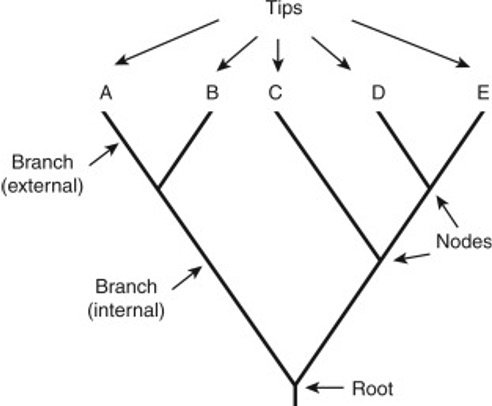
\includegraphics{Figures/slide1.jpg}
\caption{alt text}
\end{figure}

\textbf{Monophylogeny} \textbar:--------:\textbar{}
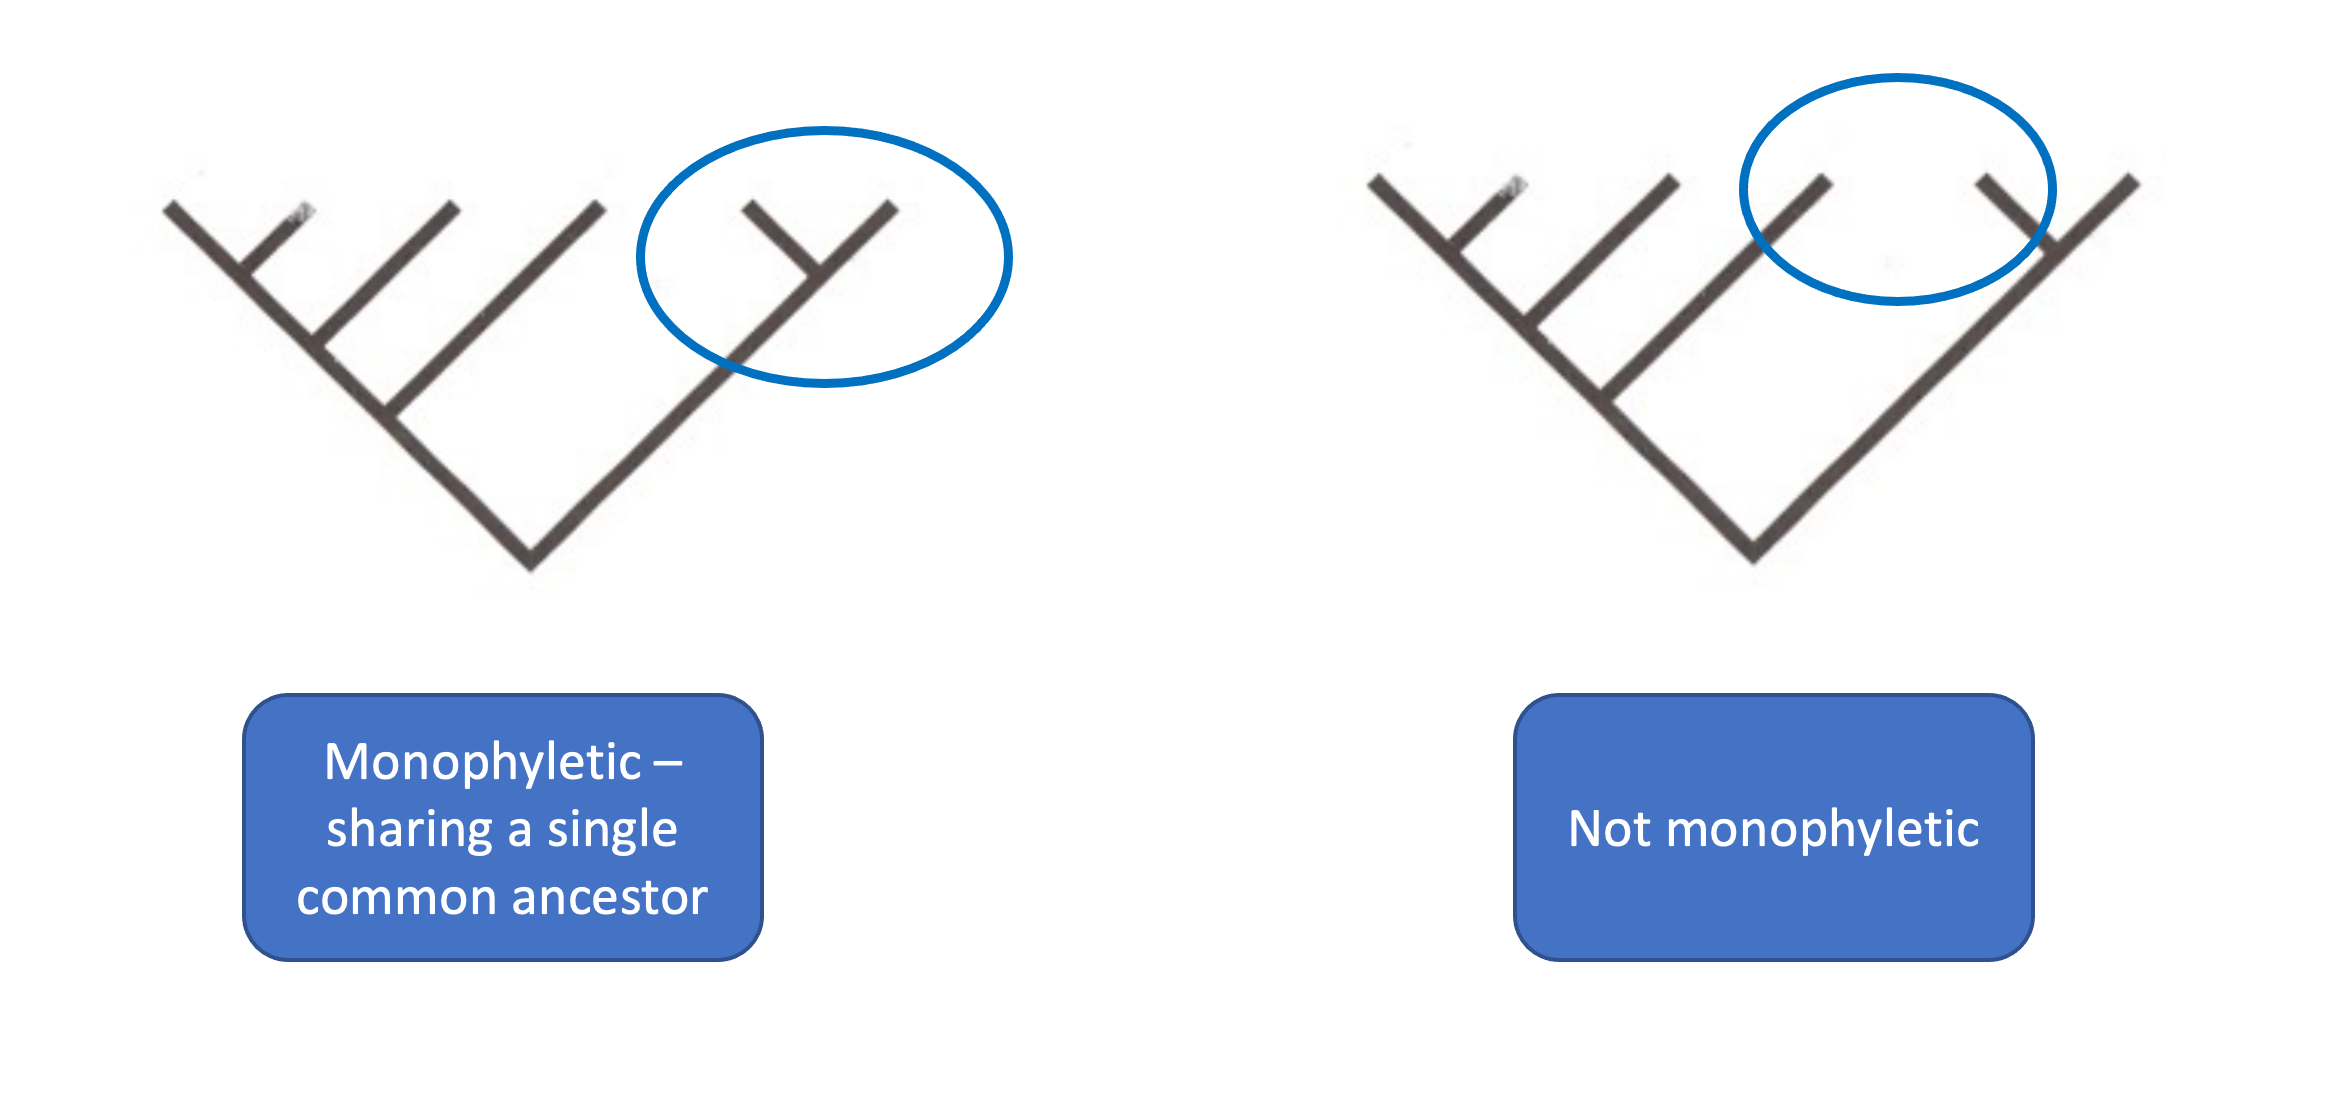
\includegraphics{Figures/slide2.png}

\textbf{Rooting Trees} \textbar:--------:\textbar{}
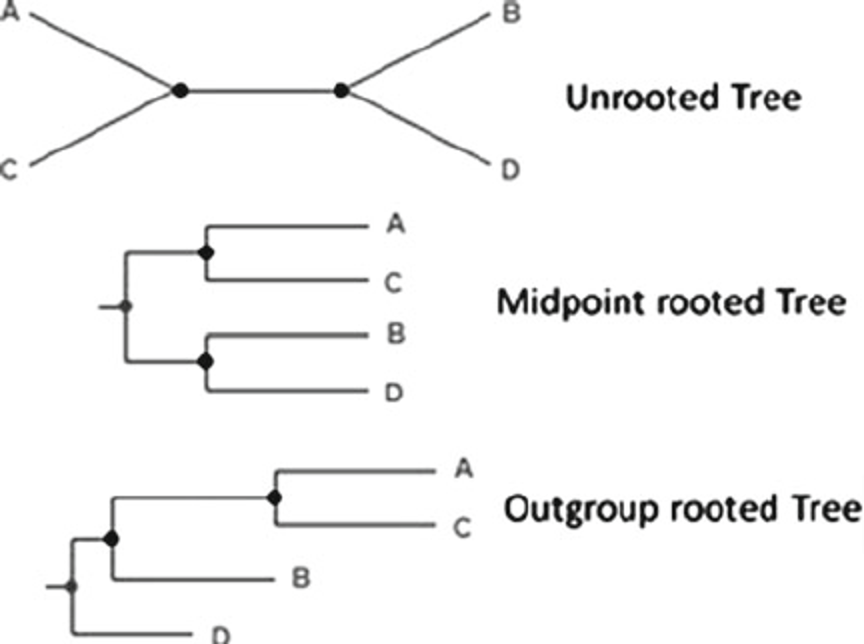
\includegraphics{Figures/slide3.png}

\textbf{Types of Tree} \textbar:--------:\textbar{}
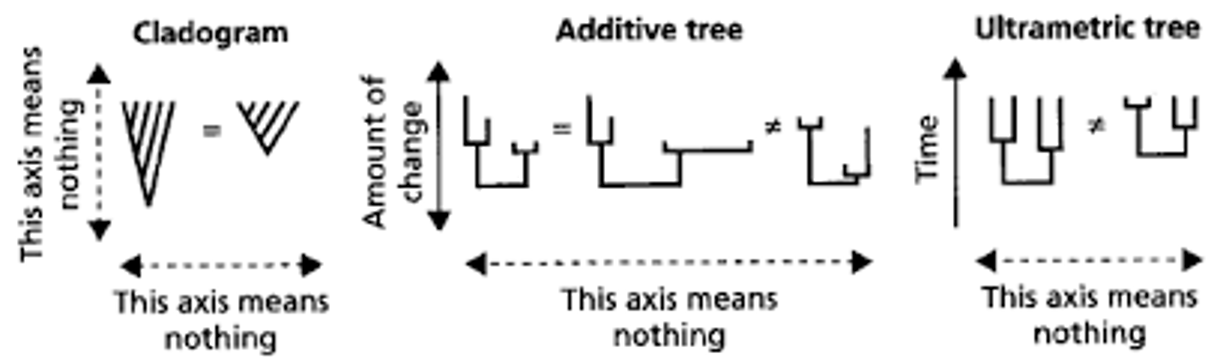
\includegraphics{Figures/slide4.png}

\hypertarget{a.1-a-simple-tree}{%
\subsection{4.2.1a.1 A Simple Tree}\label{a.1-a-simple-tree}}

We'll start off with a simple tree.

Copy the image of the tree below into a word (or other appropriate)
document. Using shapes and text boxes, annotate all of the following
answers onto the tree in the word document. \textbar:--------:\textbar{}
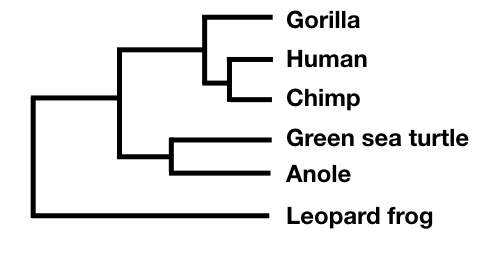
\includegraphics{Figures/figure1.png}

\begin{center}\rule{0.5\linewidth}{0.5pt}\end{center}

\hypertarget{task-1}{%
\subsubsection{Task 1}\label{task-1}}

Using an arrow and text box, label the following parts of the tree: 1.
Tip 2. Branch 3. Node

\begin{center}\rule{0.5\linewidth}{0.5pt}\end{center}

\hypertarget{task-2}{%
\subsubsection{Task 2}\label{task-2}}

Give examples of species in this tree that form: 1. A monophyletic group
2. A non-monophyletic group 3. Which of the above could be described as
a `clade'?

\begin{center}\rule{0.5\linewidth}{0.5pt}\end{center}

\hypertarget{task-3}{%
\subsubsection{Task 3}\label{task-3}}

From this tree, which is the most closely related species to Humans?
Which is most distantly related?

\begin{center}\rule{0.5\linewidth}{0.5pt}\end{center}

\hypertarget{a.2-a-more-complex-tree}{%
\subsection{4.2.1a.2 A More Complex
Tree}\label{a.2-a-more-complex-tree}}

Now we've practiced on a simple tree, can we apply the same knowledge to
a more complicated tree?

Copy the image of the tree below into a word (or other appropriate)
document. Using shapes and text boxes, annotate all of the following
answers onto the tree in the word document. \textbar:--------:\textbar{}
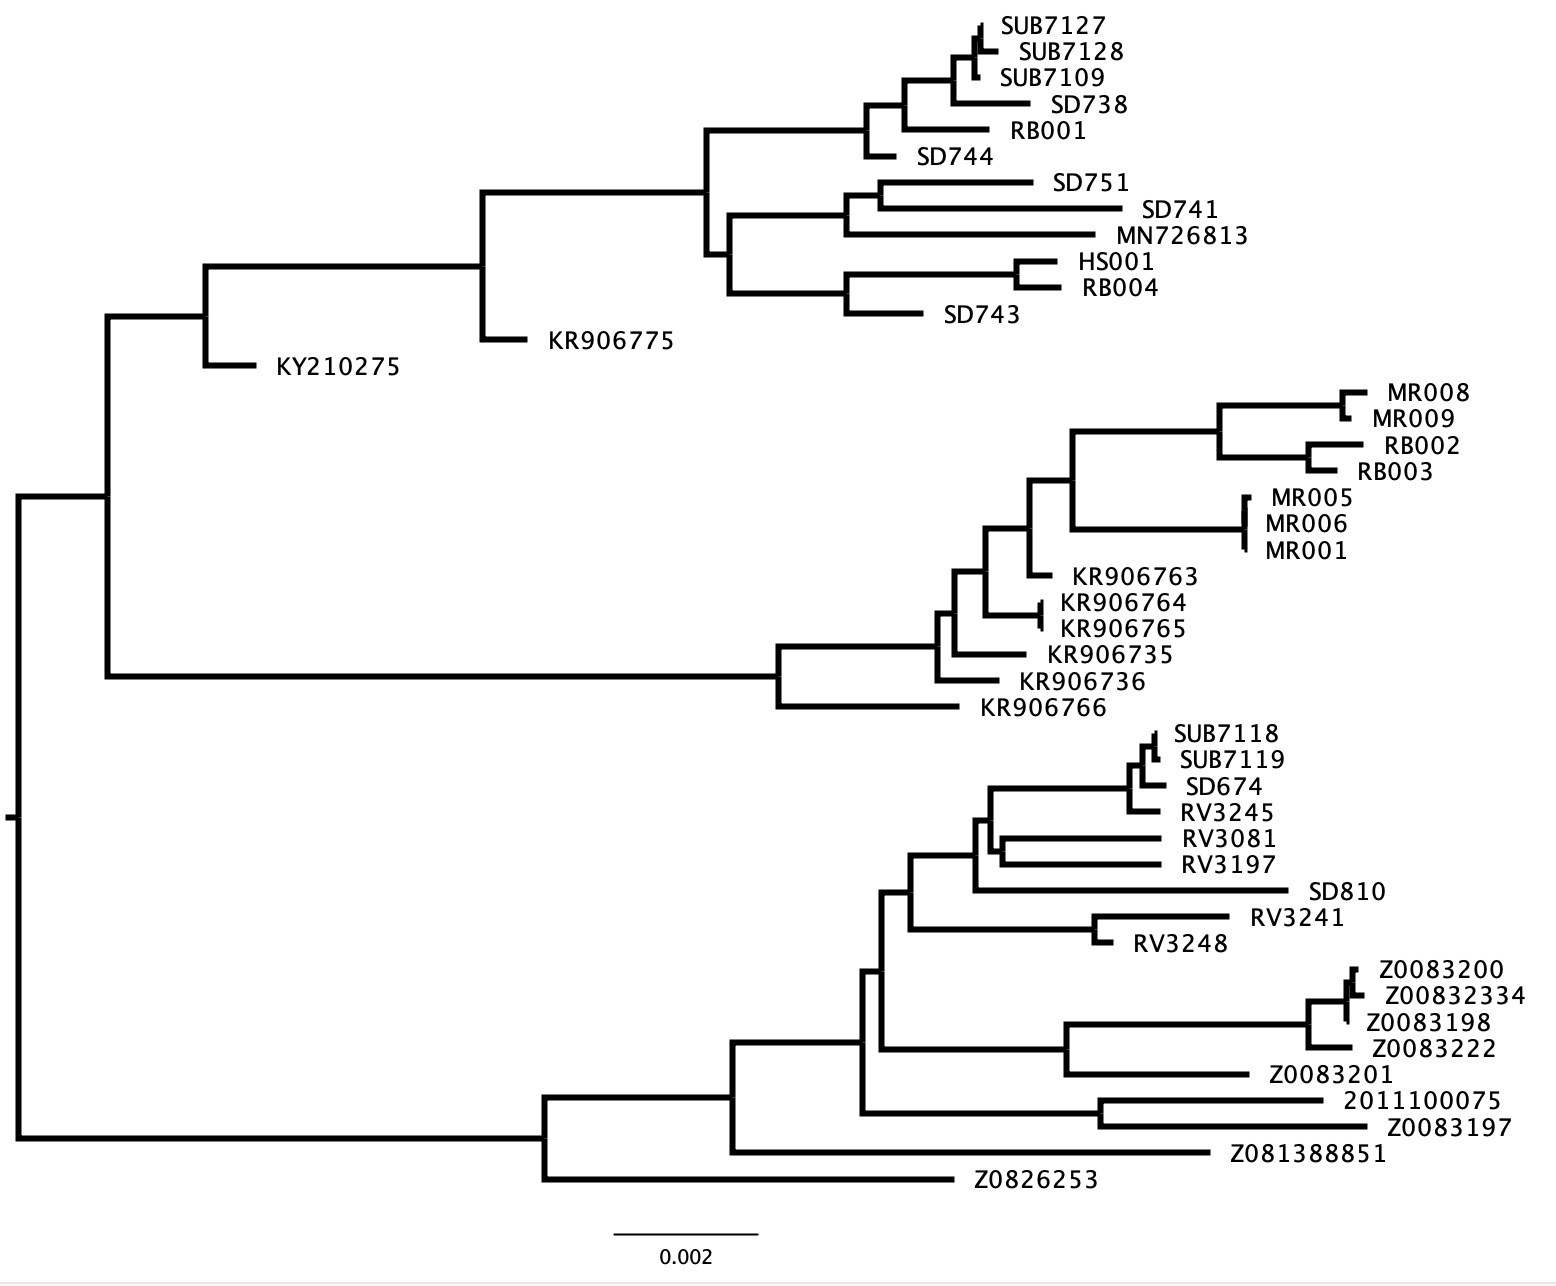
\includegraphics{Figures/figure2.png}

\begin{center}\rule{0.5\linewidth}{0.5pt}\end{center}

\hypertarget{task-3-1}{%
\subsubsection{Task 3}\label{task-3-1}}

Using an arrow and text box, label the following parts of the tree: 1.
Tip 2. Branch 3. Node 4. Root

\begin{center}\rule{0.5\linewidth}{0.5pt}\end{center}

\hypertarget{task-4}{%
\subsubsection{Task 4}\label{task-4}}

There are 3 major clades within this tree. Can you identify the nodes
that define these clades?

\begin{center}\rule{0.5\linewidth}{0.5pt}\end{center}

\hypertarget{task-5}{%
\subsubsection{Task 5}\label{task-5}}

From this tree, which sequences are most closely related to SD743?

\begin{center}\rule{0.5\linewidth}{0.5pt}\end{center}

\hypertarget{task-6}{%
\subsubsection{Task 6}\label{task-6}}

Which node represents the most recent common ancestor of sequences MR001
and KR906766?

\begin{center}\rule{0.5\linewidth}{0.5pt}\end{center}

\hypertarget{task-7}{%
\subsubsection{Task 7}\label{task-7}}

What do the branch lengths represent in this tree?

\begin{center}\rule{0.5\linewidth}{0.5pt}\end{center}

\hypertarget{a.3-types-of-tree}{%
\subsection{4.2.1a.3 Types of Tree}\label{a.3-types-of-tree}}

\begin{center}\rule{0.5\linewidth}{0.5pt}\end{center}

\hypertarget{task-8}{%
\subsubsection{Task 8}\label{task-8}}

Looking at the simple and complex trees you have in your document, which
of these appears to be outgroup rooted and which appears to be midpoint
rooted?

\begin{center}\rule{0.5\linewidth}{0.5pt}\end{center}

\hypertarget{task-9}{%
\subsubsection{Task 9}\label{task-9}}

Looking at the simple and complex trees you have in your document, which
of these appears to be an additive tree and which appears to be an
ultrametric tree? How can you tell?

\begin{center}\rule{0.5\linewidth}{0.5pt}\end{center}

\end{document}
